\section{Missbrauch des „Wo ist?“ Dienstes}
\label{sec:Missbrauch}

Das Hauptangriffsziel für Angreifer des „Wo ist?“ Dienstes sind die Standortdaten der Nutzer.
Apple ergreift verschiedene Maßnahmen, um die Sicherheit der Standortdaten sicherzustellen, wie bei der Erläuterung der Funktionsweise in \autoref{sec:Funktionsweise_FindMy} bereits gezeigt wurde.
Untersuchungen, wie durch Tonetto \textit{et al.} \cite{Tonetto_FindMy} haben jedoch geyeigt, dass dennoch Missbrauchspotenzial besteh, gegen welches der Dienst nicht oder nicht ausreichend geschützt ist.
Zunächst werden in \autoref{tab:cia_findmy} die allgemeinen Sicherheitsziele Vertraulichkeit (\textit{Confidentiality}), Integrität (\textit{Integrity}) und Verfügbarkeit (\textit{Availability}) sowie mögliche Angriffsziele im Kontext des „Wo ist?“ Dienstes erklärt.
Darauf aufbauend wird gezeigt, wie die von Apple implementierten Sicherheitsmaßnahmen, viele Angriffsszenarien erfolgreich unterbinden können.
Im Anschluss werden in \autoref{sec:szenarien} konkrete Missbrauchsszenarien aufgezeigt werden, gegen welche Apple nur unzureichende Maßnahmen ergreift und welche somit die Sicherheit und Privatsphäre der Nutzer und sogar Dritter gefährden können.
Diese Szenarien werden in \autoref{sec:Gegenmassnahmen} wieder aufgegriffen und mögliche Gegenmaßnahmen durch Apple respektive die Nutzer vorgestellt.

\begin{table}[h]
  \caption{Sicherheitsziele des „Wo ist?“ Dienstes und mögliche Angriffsziele.}
  \label{tab:cia_findmy}
  \begin{tabularx}{\textwidth}{ |l|X|X| }
    \hline
    \textbf{Sicherheitsziel}  & \textbf{Beschreibung}                                               & \textbf{Angriffsziel}                                           \\
    \Xhline{0.5mm}
    \hline
    Vertraulichkeit           & Standortdaten sind nur befugten Personen zugänglich.                & Standort eines Nutzers oder eines Geräts erhalten.              \\
    \hline
    Integrität                & Standortdaten sind vor Manipulation geschützt.                      & Standortdaten eines Nutzers oder eines Geräts manipulieren.     \\
    \hline
    Verfügbarkeit             & Standortdaten können abgerufen werden.                              & Verhindern, dass Standortdaten abgerufen werden können.         \\
    \hline
  \end{tabularx}
\end{table}

Die von Heinrich \textit{et al.} \cite{Heinrich_FindMy} identifizierten Angreifermodelle in \autoref{fig:adversary_models} zeigen verschiedene Möglichkeiten, wie ein Angreifer versuchen kann, den Dienst anzugreifen.
Sie gehen von vier verschiedenen Angreifermodellen aus, die sich im Angriffsvektor unterscheiden.
Potenzielle Angriffe können demnach von lokal installierten Anwendungen, Geräten in \ac{BLE}-Reichweite, einem klassischen Netzwerkangreifer und dem Dienstanbieter, also von Apple ausgehen.
Für jeden Angriffsvektor werden verschiedene mögliche Ziele definiert.
\begin{figure}[ht]
  \centering
  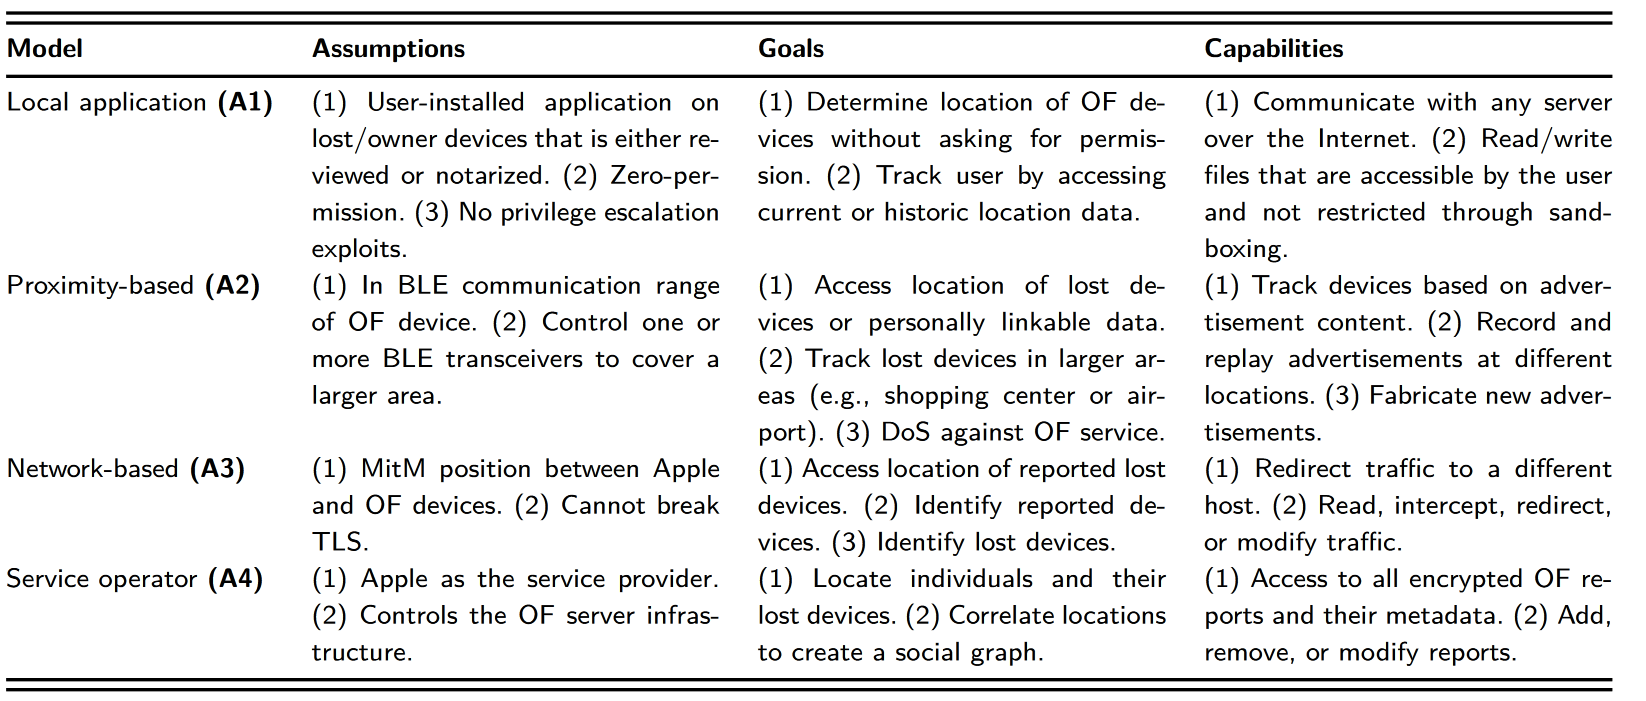
\includegraphics[width=\textwidth]{img/adversary_models}
  \caption{Angreifermodelle für den „Wo ist?“ Dienst \cite{Heinrich_FindMy}.}
  \label{fig:adversary_models}
\end{figure}

\autoref{tab:cia_adversary_models} ordnet den Zielen der einzelnen Angreifermodelle die betroffenen Sicherheitsziele zu.
\begin{table}[h]
  \caption{Zuordnung der Ziele der Angreifermodelle zu den allgemeinen Sicherheitszielen.}
  \label{tab:cia_adversary_models}
  \centering

  \begin{tabularx}{\textwidth}{ |l|X|X|l|X| }
    \hline
    \textbf{Angreifermodell}  & \textbf{Ziel} & \textbf{Vertraulichkeit} & \textbf{Integrität} & \textbf{Verfügbarkeit} \\
    \Xhline{0.5mm}
    \hline
    \multirow{2}{*}{A1} & (1) & \cmark & & \\
    \cline{2-5}
    & (2) & \cmark & & \\
    \hline
    \multirow{3}{*}{A2} & (1) & \cmark & & \\
    \cline{2-5}
    & (2) & \cmark & & \\
    \cline{2-5}
    & (3) & & & \cmark  \\
    \hline
    \multirow{3}{*}{A3} & (1) & \cmark & & \\
    \cline{2-5}
    & (2) & \cmark & & \\
    \cline{2-5}
    & (3) & \cmark & & \\
    \hline
    \multirow{2}{*}{A1} & (1) & \cmark & & \\
    \cline{2-5}
    & (2) & \cmark & & \\
    \hline
  \end{tabularx}
\end{table}
Dabei fällt auf, dass der Fokus auf der Vertraulichkeit der Daten liegt.
Sollten Angreifer Zugriff auf die Standortdaten erhalten, könnten sie diese für viele verschiedene Zwecke missbrauchen.
Zum Beispiel können diese Daten für gezielte Diskriminierung, Verfolgung und Überwachung durch Dritte oder auch durch staatliche Akteure verwendet werden.
Als personenbezogene Daten unterliegen die Standortdaten zusätzlich der \ac{DSGVO}.
Durch mögliche Rückschlüsse auf beispielsweise religiöse oder politische Überzeugungen sind Standortdaten nach Artikel 9 \ac{DSGVO} häufig auch als sensible personenbezogene Daten zu betrachten.
Deshalb ist Apple zumindest innerhalb der Europäischen Union auch verpflichtet, die Vertraulichkeit der Daten durch geeignete Maßnahmen zu schützen.
Wie bereits in \autoref{sec:Funktionsweise_FindMy} gezeigt, trifft Apple verschiedene Maßnahmen, die darauf abzielen die Vertraulichkeit zu wahren.
Die Auswirkungen dieser Maßnahmen werden in \autoref{sec:auswirkungen_sicherheitsmassnahmen} näher betrachtet.
Darüber hinaus werden in \autoref{sec:szenarien} mögliche Angriffe auf die Vertraulichkeit beschrieben, gegen welche die Sicherheitsmaßnahmen von Apple nicht ausreichend schützen.

Angriffe auf die Integrität und die Verfügbarkeit der Daten werden \cite{Heinrich_FindMy} nicht detailliert untersucht.
Nur das \textit{Proximity-based} Modell (A2 in \autoref{tab:cia_adversary_models}) zielt auch auf die Verfügbarkeit der Daten ab.
Wird die Verfügbarkeit beeinträchtigt, ist es für den Besitzer eines Geräts nicht mehr möglich, die aktuellen Standortdaten abzurufen.
Die Beeinträchtigung der Integrität der Daten wird nicht untersucht.
Jedoch ist ein gewisser Zusammenhang mit der Verfügbarkeit gegeben.
Durch gezielte Manipulation der Daten kann der Besitzer beispielsweise nicht mehr unterscheiden welche Daten korrekt sind, was die Verfügbarkeit stark beeinträchtigen kann.
Inwieweit Apples Sicherheitsmaßnahmen auch Integrität und Verfügbarkeit schützen, und welche Angriffe dennoch möglich sind, wird in \autoref{sec:auswirkungen_sicherheitsmassnahmen} und \autoref{sec:szenarien} näher betrachtet.


\subsection{Auswirkungen der Sicherheitsmaßnahmen}
\label{sec:auswirkungen_sicherheitsmassnahmen}

\subsubsection{Ende-zu-Ende Verschlüsselung}
Die Betrachtung der Funktionsweise in \autoref{sec:Funktionsweise_FindMy} zeigt, wie die Ende-zu-Ende-Verschlüsselung des Dienstes technisch umgesetzt wird.
Durch die Verwendung dieses Verschlüsselungsmechanismus kann unter der Annahme, dass der Angreifer die Verschlüsselung nicht brechen kann, gewährleistet werden, dass nur der Besitzer eines verlorenen Geräts die Standortdaten entschlüsseln kann.
Sollte einem Angreifer gelingen die Daten direkt von Apples Server abzurufen, oder über einen \ac{MITM} Angriff die verschlüsselten Daten zu erhalten, können diese ohne die nur auf den Owner Devices verfügbaren Schlüssel nicht entschlüsselt werden.
Dabei werden ein \ac{MITM}-Angriffe durch die Verwendung von \ac{TLS} mit Certificate Pinning bei der Kommunikation mit Apples Servern verhindert \cite{Heinrich_FindMy}.
Durch die Ende-zu-Ende Verschlüsselung werden alle vom Netzwerkangreifer (A3 in \autoref{fig:adversary_models}) ausgehenden Bedrohungen adressiert.
Die zur Entschlüsselung benötigten Schlüssel werden auf den Geräten des Besitzers in der als sicher geltenden iCloud Keychain gespeichert.
So werden auch die von lokalen Angreifern (A1 in \autoref{fig:adversary_models}) ausgehenden Bedrohungen behandelt.
Eine in \cite{Heinrich_FindMy} aufgedeckte Schwachstelle, die aufgrund von unsicherer Speicherung der Schlüssel unbefugten Zugriff auf die Standortdaten ermöglicht, wurde durch Apple mittlerweile behoben.
Zusätzlich wird es durch die Ende-zu-Ende-Verschlüsselung auch Apple unmöglich gemacht, auf die Standortdaten der Nutzer zuzugreifen, womit das Lokalisieren durch den Dienstanbieter (A4 mit Ziel (1) in \autoref{fig:adversary_models}) verhindert wird.
Außerdem verbessert die Verschlüsselung die Integrität der Daten, da einmal verschlüsselte Daten ohne Entschlüsselung nicht manipuliert werden können, ohne dass diese Manipulation erkannt werden kann.
Jedoch ist es möglich, dass die Standortdaten auf Basis eines Replay-Angriffes generiert wurden.
Auf dieses Szenario wird in \autoref{sec:szenarien} näher eingegangen.


\subsubsection{Schlüsselrotation}
Die Schlüsselrotation der Advertising Keys im Intervall von 15 Minuten bei Endgeräten und bis zu 24 Stunden bei Accesories, wie in \autoref{sec:Funktionsweise_FindMy} beschrieben, trägt ebenfalls zur Vertraulichkeit der Standortdaten bei.
Durch die regelmäßige Rotation der Schlüssel wird das Tracking von Geräten anhand der im Advertising gesendeten Daten erschwert.
Damit richtet sich diese Maßnahme gezielt gegen das Tracking durch einen Angreifer in der Nähe (A2 mit Ziel (2) in \autoref{fig:adversary_models}).
Außerdem müssten für einen solchen Angriff viele scannende Geräte so positioniert werden, dass auch bei Bewegung die Advertisement Pakete des zu verfolgenden Geräts von einem der Scanner erfasst wird.
Um größere Bereiche abzudecken, wären jedoch sehr viele scannende Geräte notwendig, was den Angriff bereits deutlich erschwert.
In Verbindung mit der Schlüsselrotation ist die Verfolgung, auch mit hohem Aufwand, nur für das Intervall der Schlüsselrotation möglich.
Allerdings können AirTags und Drittanbieterprodukte durch das längere Intervall für bis zu 24 Stunden über einen solchen Angriff verfolgt werden.
Für Angreifer ist der Angriff jedoch insgesamt so komplex, dass eine direkte Verfolgung des Opfers in den meisten Fällen praktikabler wäre.
Heinrich \textit{et al.} \cite{Heinrich_FindMy} betrachten die Schlüsselrotation als ausreichend, um die Verfolgung von Geräten nach diesem Muster zu verhindern.
Jedoch waren zum Zeitpunkt ihrer Analyse keine Geräte mit einem Intervall der Schlüsselrotation von mehr als 15 Minuten auf dem Markt.


\subsection{Missbrauchsszenarien ohne ausreichende Gegenmaßnahmen}
\label{sec:szenarien}

Im Folgenden sind sieben Missbrauchsszenarien aufgeführt, welche nicht ausreichend durch Gegenmaßnahmen unterbunden werden.
Gegen einige werden gar keine Maßnahmen getroffen, andere Gegenmaßnahmen lassen sich leicht umgehen und sind dementsprechend nicht ausreichend.
Weiterhin ist Szenario \nameref{missbrauch:4} nicht als negativer Missbrauch zu verstehen, da der „Wo ist?“ Dienst in diesem Fall nicht zur Beeinträchtigung, sondern zur Steigerung der Privatsphäre genutzt wird.
Weil dieser Anwendungsfall jedoch nicht von Apple vorgesehen ist, handelt es sich dennoch um Missbrauch.
Die Szenarien basieren größtenteils auf den Arbeiten von Heinrich \textit{et al.} \cite{Heinrich_FindMy}, Tonetto \textit{et al.} \cite{Tonetto_FindMy}, Mayberry \textit{et al.} \cite{Mayberry_Tracking} und Garg \textit{et al.} \cite{Garg_Secure_Tracker}.

\subsubsection[M1]{M1: Replay-Angriff}
\label{missbrauch:1}
Durch die Ende-zu-Ende-Verschlüsselung und den authentifizierten Upload der Standortdaten, kann die Integrität der Standortdaten in vielen Fällen geschützt werden.
Allerdings können über einen Replay-Angriff manipulierte Standortdaten, welche korrekt verschlüsselt sind und authentifiziert hochgeladen werden, auf Apples Server gelangen.
Somit kann die Integrität der abgerufenen Standortdaten nicht mehr gewährleistet werden.
Der Nutzer kann eventuell nicht mehr erkennen, welche Daten korrekt sind und kann somit keine verlässliche Standortinformation erhalten, was die Verfügbarkeit beeinträchtigt \cite{Heinrich_FindMy}.
Dieser Angriff entspricht dem \ac{DOS}-Angriff durch einen Angreifer in der Nähe (A2 mit Ziel (3) in \autoref{fig:adversary_models}).

Um einen solchen Angriff durchzuführen, kann ein Angreifer die Advertisement Pakete eines Gerätes aufzeichnen und an anderen Orten wieder abspielen.
Geräte in der Nähe empfangen diese Pakete und senden Standortdaten verschlüsselt und korrekt authentifiziert an Apple.
Der Besitzer erhält die manipulierten Standortdaten interpretiert diese als korrekt, oder kann nicht mehr erkennen, welche Daten korrekt sind.
Es ist unklar, ob Apple gegen diese Art der Manipulation Maßnahmen ergreift.


\subsubsection[M2.1]{M2.1: \ac{DOS}: Angreifer mit physischem Zugriff}
\label{missbrauch:2.1}
Die Verfügbarkeit der Standortdaten ist für die Betrachtung im Rahmen dieser Arbeit weniger relevant, da das Design des Dienstes vergleichsweise wenige Auswirkungen auf die Verfügbarkeit hat.
Dennoch ist die Verfügbarkeit durch verschiedene Angriffe bedroht.
Zum Beispiel könnte ein direkter \ac{DOS} Angriff auf die Server von Apple erfolgen, was allerdings als unwahrscheinliches Bedrohungsszenario angesehen werden kann.
Relevanter ist ein Angriff durch einen Angreifer mit physischem Zugriff auf das Lost Device.
Beispielsweise in Zusammenhang mit Diebstahl eines Gegenstandes, an welchem ein AirTag befestigt ist, kann durch Zerstörung oder Entfernen der Batterie, verhindert werden, dass neue Standortinformationen hochgeladen werden.
In diesem Kontext ist auch das Entfernen des AirTags vom Gegenstand möglich um die weitere Lokalisierung zu verhindern.
Da keine neuen, gültigen Standortdaten erzeugt werden, ist die Verfügbarkeit eingeschränkt.

\subsubsection[M2.2]{M2.2: \ac{DOS}: Angreifer in der Nähe}
\label{missbrauch:2.2}
Zur Einschränkung der Verfügbarkeit der Standortdaten, reicht es auch aus, wenn ein Angreifer sich in der Nähe des Geräts befindet.
Zum Beispiel ist bei dem von Garg \textit{et al.} \cite{Garg_Secure_Tracker} als sicher vorgeschlagenen Systemen neben dem Entfernen der Batterie auch das gezielte Entladen dieser ohne physischen Zugriff möglich.
Dieses System ist so gestaltet, dass der aktuelle Standort vom Finder Device an das Lost Device gesendet wird, welches die Daten verschlüsselt zurückgibt.
In diesem Szenario kann ein Angreifer durch häufiges senden von Standorten an das Lost Device unter Zuhilfenahme der energieintensiven Verschlüsselungsoperationen, die Batterie des Lost Devices entladen.
Ein Angriff nach diesem Schema kann auch Apples System betreffen.
Insbesondere für Accessories geringer Batteriekapazität ist die gezielte Entladung ein relevantes Bedrohungsszenario.
Da jedoch beim „Wo ist?“ Dienst die Verschlüsselung nicht auf dem Lost Device erfolgt, muss der Angriff leicht variiert werden.
Accessories müssen die Möglichkeit bieten, einen Ton abzuspielen \cite{Apple_FindMySpec}.
Diese Funktion kann durch jeden in \ac{BLE}-Reichweite ausgelöst werden \cite{Heinrich_AirGuard} und genutzt werden, um die Batterie zu entladen.

\subsubsection[M3]{M3: Direktes Tracking von Personen}
\label{missbrauch:3}
Das Szenario des direkten Trackings von Personen bezieht sich auf die Verfolgung durch AirTags oder andere kleine Tracker.
Durch die kleine Größe der Tracker können diese in Jacken, Rucksäcken oder an Fahrzeugen befestigt werden, um einzelne Personen gezielt zu verfolgen \cite{Roth_airtags}.
Dieser Angriff wurde bereits vielfach in der Praxis beobachtet und für Stalking oder Autodiebstahl genutzt \cite{NYT_Airtags}.
Der „Wo ist?“ Dienst bietet zwar eine Funktion zur \ac{UT}, um Nutzer auf mögliche Verfolgung hinzuweisen \cite{Apple_FindMySpec}.
Allerdings wurde bereits gezeigt, dass diese Funktion leicht umgangen werden kann \cite{Mayberry_Tracking} und in vielen Fällen nicht zuverlässig vor Tracking warnen kann \cite{Heinrich_AirGuard}.
Darüber hinaus ist die Funktion nur für iOS-Geräte direkt verfügbar, sodass für Android-Nutzer keinerlei Warnung erfolgt.
Demnach sind die Gegenmaßnahmen des „Wo ist?“ Dienstes gegen das direkte Tracking von Personen als nicht ausreichend zu bewerten.


\subsubsection[M4]{M4: Indirektes Tracking von Personen}
\label{missbrauch:4}
Beim indirekten Tracking werden Personen nicht durch Tracker direkt verfolgt.
Stattdessen werden anhand der Uploadzeitpunkte von Location Reports Rückschlüsse auf die Bewegung von Personen gezogen.
Dieses Missbrauchsszenario wurde von Tonetto \textit{et al.} \cite{Tonetto_FindMy} vorgestellt und kann nicht nur für das schadhafte Tracking von Personen genutzt werden, sondern auch zum Crowd-Monitoring unter Wahrung der Privatsphäre.
Da Finder Devices Location Reports generell gebündelt hochladen, und Apples Server die Uploadzeitpunkte mit einer Genauigkeit von wenigen Millisekunden speichern, können Angreifer Location Reports, die vom gleichen Gerät stammen miteinander in Verbindung zu bringen \cite{Tonetto_FindMy}.
Während Finder Devices mit Mobilfunkverbindung Location Reports in der Regel erst nach einigen Stunden hochladen, erfolgt der Upload bei einer WLAN-Verbindung deutlich schneller.
Wechselt ein Finder Device von einer Mobilfunkverbindung zu einer WLAN-Verbindung, werden die zwischengespeicherten Location Reports in der Regel kurz darauf hochgeladen.
Unter der Annahme, dass Personen außerhalb einiger weniger Orte, wie zum Beispiel der eigenen Wohnung, nicht dauerhaft mit einem WLAN-Netzwerk verbunden sind, werden außerhalb dieser Orte erstellte Location Reports in etwa zur gleichen Zeit hochgeladen \cite{Tonetto_FindMy}.

Platziert ein Angreifer mehrere Tracker an verschiedenen Orten, erfassen Finder Devices diese und generieren jeweils Location Reports.
Jeder dieser Location Reports gibt an, zu welchem Zeitpunkt das Finder Device an welcher Position war.
Werden diese Location Reports gebündelt hochgeladen, kann der Angreifer die zusammengehörigen Location Reports anhand der Uploadzeitpunkte identifizieren.
Aus den Positionen und Zeitpunkten der Erstellung der Reports kann die Bewegung des Finder Device rekonstruiert werden \cite{Tonetto_FindMy}.


Zur Nutzung zum Crowd-Monitoring werden einzelne Tracker an öffentlichen Orten platziert.
Finder Devices, die sich in der Nähe dieser Tracker befinden, generieren Location Reports für diese.
Diese Reports können von Apples Servern heruntergeladen werden und erlauben über die Anzahl der Reports für einen bestimmten Tracker Rückschlüsse auf die Anzahl der iPhone-Nutzer, die sich in der Nähe des Trackers aufgehalten haben.
Die Zahl der iPhone-Nutzer kann verwendet werden, um die Gesamtzahl der Personen zu schätzen, beispielsweise unter Einbeziehung eines KI-Systems.
Durch die Verzögerung beim Upload der Reports sind die Daten allerdings ebenfalls nur mit einer gewissen Verzögerung verfügbar \cite{Tonetto_FindMy}.

Über die Verwendung mehrere Tracker lassen sich auch die Bewegungen von Menschenmengen rekonstruieren.
Dabei werden die Tracker an verschiedenen Orten platziert und die Location Reports der Finder Devices heruntergeladen.
Anhand der Uploadzeitpunkte der Reports kann bestimmt werden, welche Reports vom gleichen Finder Device stammen \cite{Tonetto_FindMy}.
Darauf aufbauend kann die Zeit bestimmt werden, die das Finder Device benötigt hat, die Distanz zwischen jeweils zwei Trackern zurückzulegen.
Alternativ könnte, über das oben vorgestellte Verfahren, die Anzahl der Personen in der Nähe jedes Trackers zu verschiedenen Zeiten bestimmt werden und auf Basis der Veränderungen Rückschlüsse auf die Bewegungen der Menschenmengen gezogen werden.


Dieser Missbrauch des „Wo ist?“ Dienstes kann als Alternative zu aktuellen Crowd-Monitoring-Systemen, welche auf Bilderkennung oder der Auswertung von Wi-Fi Management Frames basieren, verwendet werden und erlaubt eine ähnliche Genauigkeit.
Zusätzlich ist dieser Ansatz besser für die Privatsphäre der Betroffenen, da keine personenbezogenen Daten erhoben werden \cite{Tonetto_FindMy}.
Deshalb wird dieser Einsatzzweck als „positiver“ Missbrauch des „Wo ist?“ Dienstes bewertet.


\subsection[M5]{M5: Verdeckter Datentransfer}
\label{missbrauch:5}
Tonetto \textit{et al.} \cite{Tonetto_FindMy} und Bräunlein \cite{braeunlein_sendmy} zeigen unabhängig voneinander, dass der „Wo ist?“ Dienst auch für einen verdeckten Datentransfer mit einer niedrigen Übertragungsrate ausgenutzt werden kann.
Dabei werden Finder Devices dazu genutzt, Daten an Apples Server zu übertragen, welche vom Angreifer heruntergeladen und dekodiert werden können.
Beide verwenden für das Senden der Daten einen Nachbau eines AirTags, bestehend aus einem \ac{BLE}-fähigen Mikrocontroller.

Bräunlein \cite{braeunlein_sendmy} kodiert eine zu sendende Nachricht in den im Advertisement gesendeten Daten.
Für jedes Bit der Nachricht wird ein 28 Byte langes Array, bestehend aus der Position des Bits in der Nachricht, einer ID des Senders und dem Wert des Bits generiert.
Anstatt einen öffentlichen Schlüssel im Advertisement zu senden, werden die so kodierten Daten für eine definierte Zeitspanne gesendet.
Danach wird der Prozess für das nächste Bit der Nachricht wiederholt.
Diese Kodierung ist in \autoref{fig:sendmy_encoding} schematisch dargestellt.
\begin{figure}[ht]
  \centering
  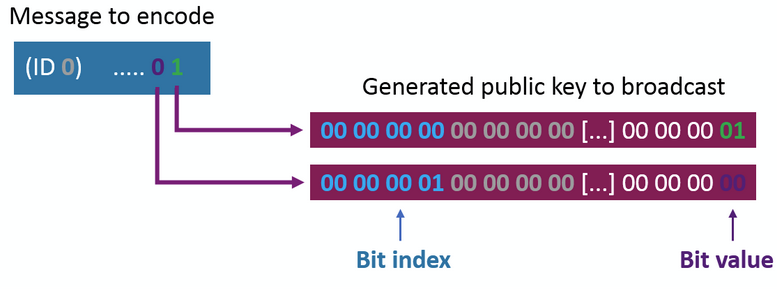
\includegraphics[width=0.9\linewidth]{sendmy_encoding.png}
  \caption{Bitweise Kodierung der Nachricht in im Advertisement übertragenen Daten \cite{braeunlein_sendmy}.}
  \label{fig:sendmy_encoding}
\end{figure}
Der Empfänger kann für jedes Bit der Nachricht die zwei möglichen Arrays generieren und eine Anfrage mit den jeweiligen \ac{SHA}-256 Hashes an Apples Server senden.
Abhängig davon, welcher der beiden Hashes in der Antwort enthalten ist, kann der Empfänger das Bit der Nachricht bestimmen.
Dabei wird ausgenutzt, dass jedes Apple Gerät die verschlüsselten Location Reports für beliebige öffentliche Schlüssel herunterladen kann.
Da die Location Reports Ende-zu-Ende verschlüsselt sind, wird dadurch die Vertraulichkeit nicht gefährdet.
Jedoch ist für dieses Missbrauchszenario die Entschlüsselung der Daten nicht notwendig, da lediglich das Vorhandensein eines bestimmten Location Reports überprüft werden muss, um die Nachricht zu dekodieren.
Ein Nachteil bei diesem Verfahren ist, dass somit auch jedes Apple-Gerät die Nachricht abrufen könnte.


Das von Tonetto \textit{et al.} \cite{Tonetto_FindMy} vorgestellte Verfahren verwendet 16 bekannten Advertising Keys, um die Nachricht in eine Folge dieser Keys zu kodieren.
Dazu wird eine Menge von Advertising Keys zuvor generiert und zwischen Sender und Empfänger ausgetauscht.
Der Sender kann die Nachricht erzeugt aus der Nachricht eine Abfolge der Advertising Keys und sendet diese nacheinander im Advertisement.
Finder Devices, die sich in der Nähe befinden, empfangen die Advertisements, erstellen Location Reports und laden diese hoch.
Der Empfänger der Nachricht kann alle Location Reports der bekannten Advertising Keys herunterladen, die Daten entschlüsseln und anhand der Zeitstempel die Folge und damit die ursprüngliche Nachricht rekonstruieren.
Im Vergleich zum Verfahren von Bräunlein, werden hier echte Advertising Keys verwendet, sodass die Location Reports entschlüsselt werden können, sodass der Standort des Senders bestimmt werden kann.
Zusätzlich muss der Empfänger weniger Anfragen an Apples Server stellen, da nur 16 unterschiedliche Advertising Keys verwendet werden.
Bräunleins Verfahren benötigt zwei Anfragen an Apples Server pro übertragenem Bit.


\subsection[M6]{M6: Korrelation von Standorten durch Apple}
\label{missbrauch:6}

Das zweite Ziel des Angreifermodells des Dienstanbieters (A4 in \autoref{fig:adversary_models}) bezieht sich auf die Korrelation von Standorten mehrerer Nutzer.
Heinrich \textit{et al.} \cite{Heinrich_FindMy} zeigen, dass durch den authentifizierten Up- und Download, die Korrelation durch Apple theoretisch möglich ist.
Die konkreten Standorte können aufgrund der Ende-zu-Ende-Verschlüsselung nicht bestimmt werden.
Allerdings kann bestimmt werden, welches Gerät welche Location Reports erstellt und welcher Nutzer diese heruntergeladen hat.
Daraus lässt sich folgern, welche Nutzer sich zu welcher Zeit an einem gemeinsamen Ort aufgehalten haben.
Apple könnte diese Informationen nutzen, um soziale Beziehungen zwischen Nutzern zu bestimmen und diese, zum Beispiel zu Werbezwecken, zu analysieren.
In \cite{Heinrich_FindMy} wird zusätzlich aufgezeigt, dass diese Daten auch von Strafverfolgungsbehörden genutzt werden könnten, um unter anderem die Identität von Demonstrationsteilnehmern zu bestimmen.
Jedoch ist nicht klar, ob Apple diese Daten tatsächlich speichert und nutzt.
% TODO: weiter darauf eingehen; auch: wie ist die Rechstlage z.B. in den USA?




%TODO: sinnvoll?
\subsection{Zusammenfassung Missbrauchsszenarien ohne ausreichende Gegenmaßnahmen}
In \autoref{tab:missbrauchsszenarien} werden die Missbrauchsszenarien zusammengefasst, gegen welche von Apple aktuell keine ausreichenden Gegenmaßnahmen ergriffen werden.
Dazu sind die Zielsetzung des Angreifers und mögliche Betroffene eines solchen Angriffs aufgeführt

\begin{table}[ht]
  \caption{Zusammenfassung der Missbrauchsszenarien \nameref{missbrauch:1} bis \nameref{missbrauch:6}.}
  \label{tab:missbrauchsszenarien}
  \begin{tabularx}{\textwidth}{ |l|X|X|X| }
    \hline
    \textbf{Szenario} & \textbf{Beschreibung} & \textbf{Angriffsziel} & \textbf{Betroffene}\\
    \Xhline{0.5mm}
    \hline
    \nameref{missbrauch:1} & Replay-Angriff & Integrität, Verfügbarkeit & Nutzer des „Wo ist?“ Dienstes \\
    \hline
    \nameref{missbrauch:2.1} & \ac{DOS}: Angreifer mit physischer Zugriff & Verfügbarkeit & Nutzer des „Wo ist?“ Dienstes \\
    \hline
    \nameref{missbrauch:2.2} & \ac{DOS}: Angreifer in der Nähe & Verfügbarkeit & Nutzer des „Wo ist?“ Dienstes \\
    \hline
    \nameref{missbrauch:3} & Direktes Tracking & Vertraulichkeit & Jeder \\
    \hline
    \nameref{missbrauch:4} & Indirektes Tracking & Vertraulichkeit & Nutzer des „Wo ist?“ Dienstes  \\
    \hline
    \nameref{missbrauch:5} & Verdeckter Datentransfer & Ausnutzung zur Datenübertragung & Apple \\
    \hline
    \nameref{missbrauch:6} & Korrelation von Nutzerstandorten & Vertraulichkeit & Nutzer des „Wo ist?“ Dienstes \\
    \hline
  \end{tabularx}
\end{table}
